\documentclass[12pt, notitlepage]{article}   	
\usepackage[top=1in, bottom=1in, left=1in, right=1in]{geometry}
\usepackage{amsmath}
\usepackage{amssymb}
%\usepackage{mdwlist}
\usepackage{parskip}
%\usepackage{paralist}
\usepackage{hyperref}
\usepackage{cite} 
\usepackage{siunitx}  
\usepackage{graphicx}
\usepackage{caption}
\usepackage{subcaption}
\usepackage{color}
\usepackage{float}    %\begin{figure}[H]

\usepackage{titling}    % lower the title 
%\setlength{\droptitle}{5cm}

% comment
\newcommand{\mw}[1]{{\color{magenta} (Mingjian's Comment: #1)}}
% reference 
\newcommand{\fref}[1]{Fig.~\ref{#1}}
\newcommand{\tabref}[1]{Table~\ref{#1}}
\newcommand{\eqnref}[1]{Eq.~(\ref{#1})}
% roman number
\makeatletter
\newcommand*{\rom}[1]{\expandafter\@slowromancap\romannumeral #1@}
\makeatother


\title{\textbf{Retinal Blood Vessel Detection Method Using Machine Learning Algorithm}}
\author{Mingjian Wen (wenxx151) and Yuchen Luo (luoxx364)}
\date{}		

\begin{document}					
\maketitle
\thispagestyle{empty}
%\newpage
\setcounter{page}{1}

\begin{abstract}
\noindent Retinal vessel examination plays an important role in the diagnosis of diabetes, a leading cause of blindness in the western countries.  The examination employs the optical diagnostic method by taking digital images of the eyeball without intruding or harming people’s body.  The task remains to separate the retinal vessels from the digital images.  It is time-consuming and challenging even for trained specialists.  Machine learning methods have been introduced to automate the separation procedure so as to increase the efficiency of the examination process.  In this report, we explored the retinal vessel separation process with a combination of image processing and machine learning methods. Image preprocessing is used to reduce the noise in the raw eyeball image.  Machine learning algorithm is used to construct a classifier which takes advantage of specialist's hand-drawn retinal vessels as training label to separate the vessel from the background efficiently. K-nearest neighbor (K-NN) and Support Vector Machine (SVM) are implemented, and a modified K-NN method is used to improve the result.  Different definitions of distance in the K-NN methods are used to find the importance of different features of eye vessel image.  The errors are estimated by comparing the algorithm classified labels with the specialist's hand-drawn image. K-NN is self-coded Matlab program by using the knowledge learned in the class, and SVM is understood in the theoretical level and implemented with PyML (a python based machine learning package). The error rate of both methods are around 6\%. K-NN yields slightly better results compared SVM, and a better result is achieved by modified K-NN.  Different distance definition influences the result of the segmentation slightly. Possible Improvement of the strategies of the machine learning methods are discussed in the report as well.
\end{abstract}


\newpage
%%% sec: intro
\section{Introduction}

Diabetes is one of the top causes for blindness in the western countries \cite{centers2011national}. The earlier to diagnose it, the higher possibility to save the patients from blindness.  The process to get diabetes is slow and has no significant symptom, thus it is hard to be diagnosed and dealt with properly.  One of the most efficient way to diagnose is by inspecting the structure of blood vessels in the eyes \cite{hoover2003locating}.  When the geometric shape (e.g. length, width, and curvature) of the blood vessels shows some certain features, it indicates that there is a concern of the disease.  


The diagnostic procedure is easy to carry out, without any intrusion or pain.  First, a high quality eyeball image needs to be taken. Then, the eye vessel information is collected from the image. Based on the eye vessel information, doctors can infer whether a patient is prone to diabetes.  The vessel information is usually obtained manually by trained specialists.  It is quite a challenge task because the vessels sometimes are not easy to be distinguished from the background of the eyeball.  Thus it highly depends on the experience of the specialists.  Even for an experienced specialist, the process of segmentation takes quite a long time.  In order to increase the efficiency of segmentation work and provide the public a way to self-examine eye vessel related diseases, an automatic method is needed.  
  
There are extensive work related to this process already, and basically they fall into two categories \cite{marin2011new}.  One kind is called image processing method, including filtering, tracking, threshold probing and morphology \cite{marin2011new}. Some of these methods can be found in the \verb|Matlab| image processing toolbox.   This kind of method introduces some assumptions and needs some parameters to be setup in order to process the image. Another category is called machine learning algorithm, especially non-parametric machine learning algorithms.  This report focuses on retinal vessel segmentation using the machine learning methods, but we still use image preprocessing to get rid of some noise in the eyeball image.  

  
The goal of this report is to apply machine learning knowledge learned in CSCI 5521 into a biomedical application scenario.  We studied different classification methods, including K-nearest neighbor (K-NN), support vector machine (SVM) and a slightly modified K-NN.The optimal parameters for these methods are determined in this work. By implementing these methods, we have obtained a better understanding of the context taught in class.  The structure of the report is organized as follows: in Section~2, we discuss the data source of the eyeball images and the techniques used to to the preprocessing. Section~3 discusses the classification methods. The results are presented in Section~4 and we end the report with a discussion of pros and cons of each method in Section~5.  \fref{fig:procedure_project} shows the basic procedures of this report. 
 
 %single figure
\begin{figure}[h]
\centering
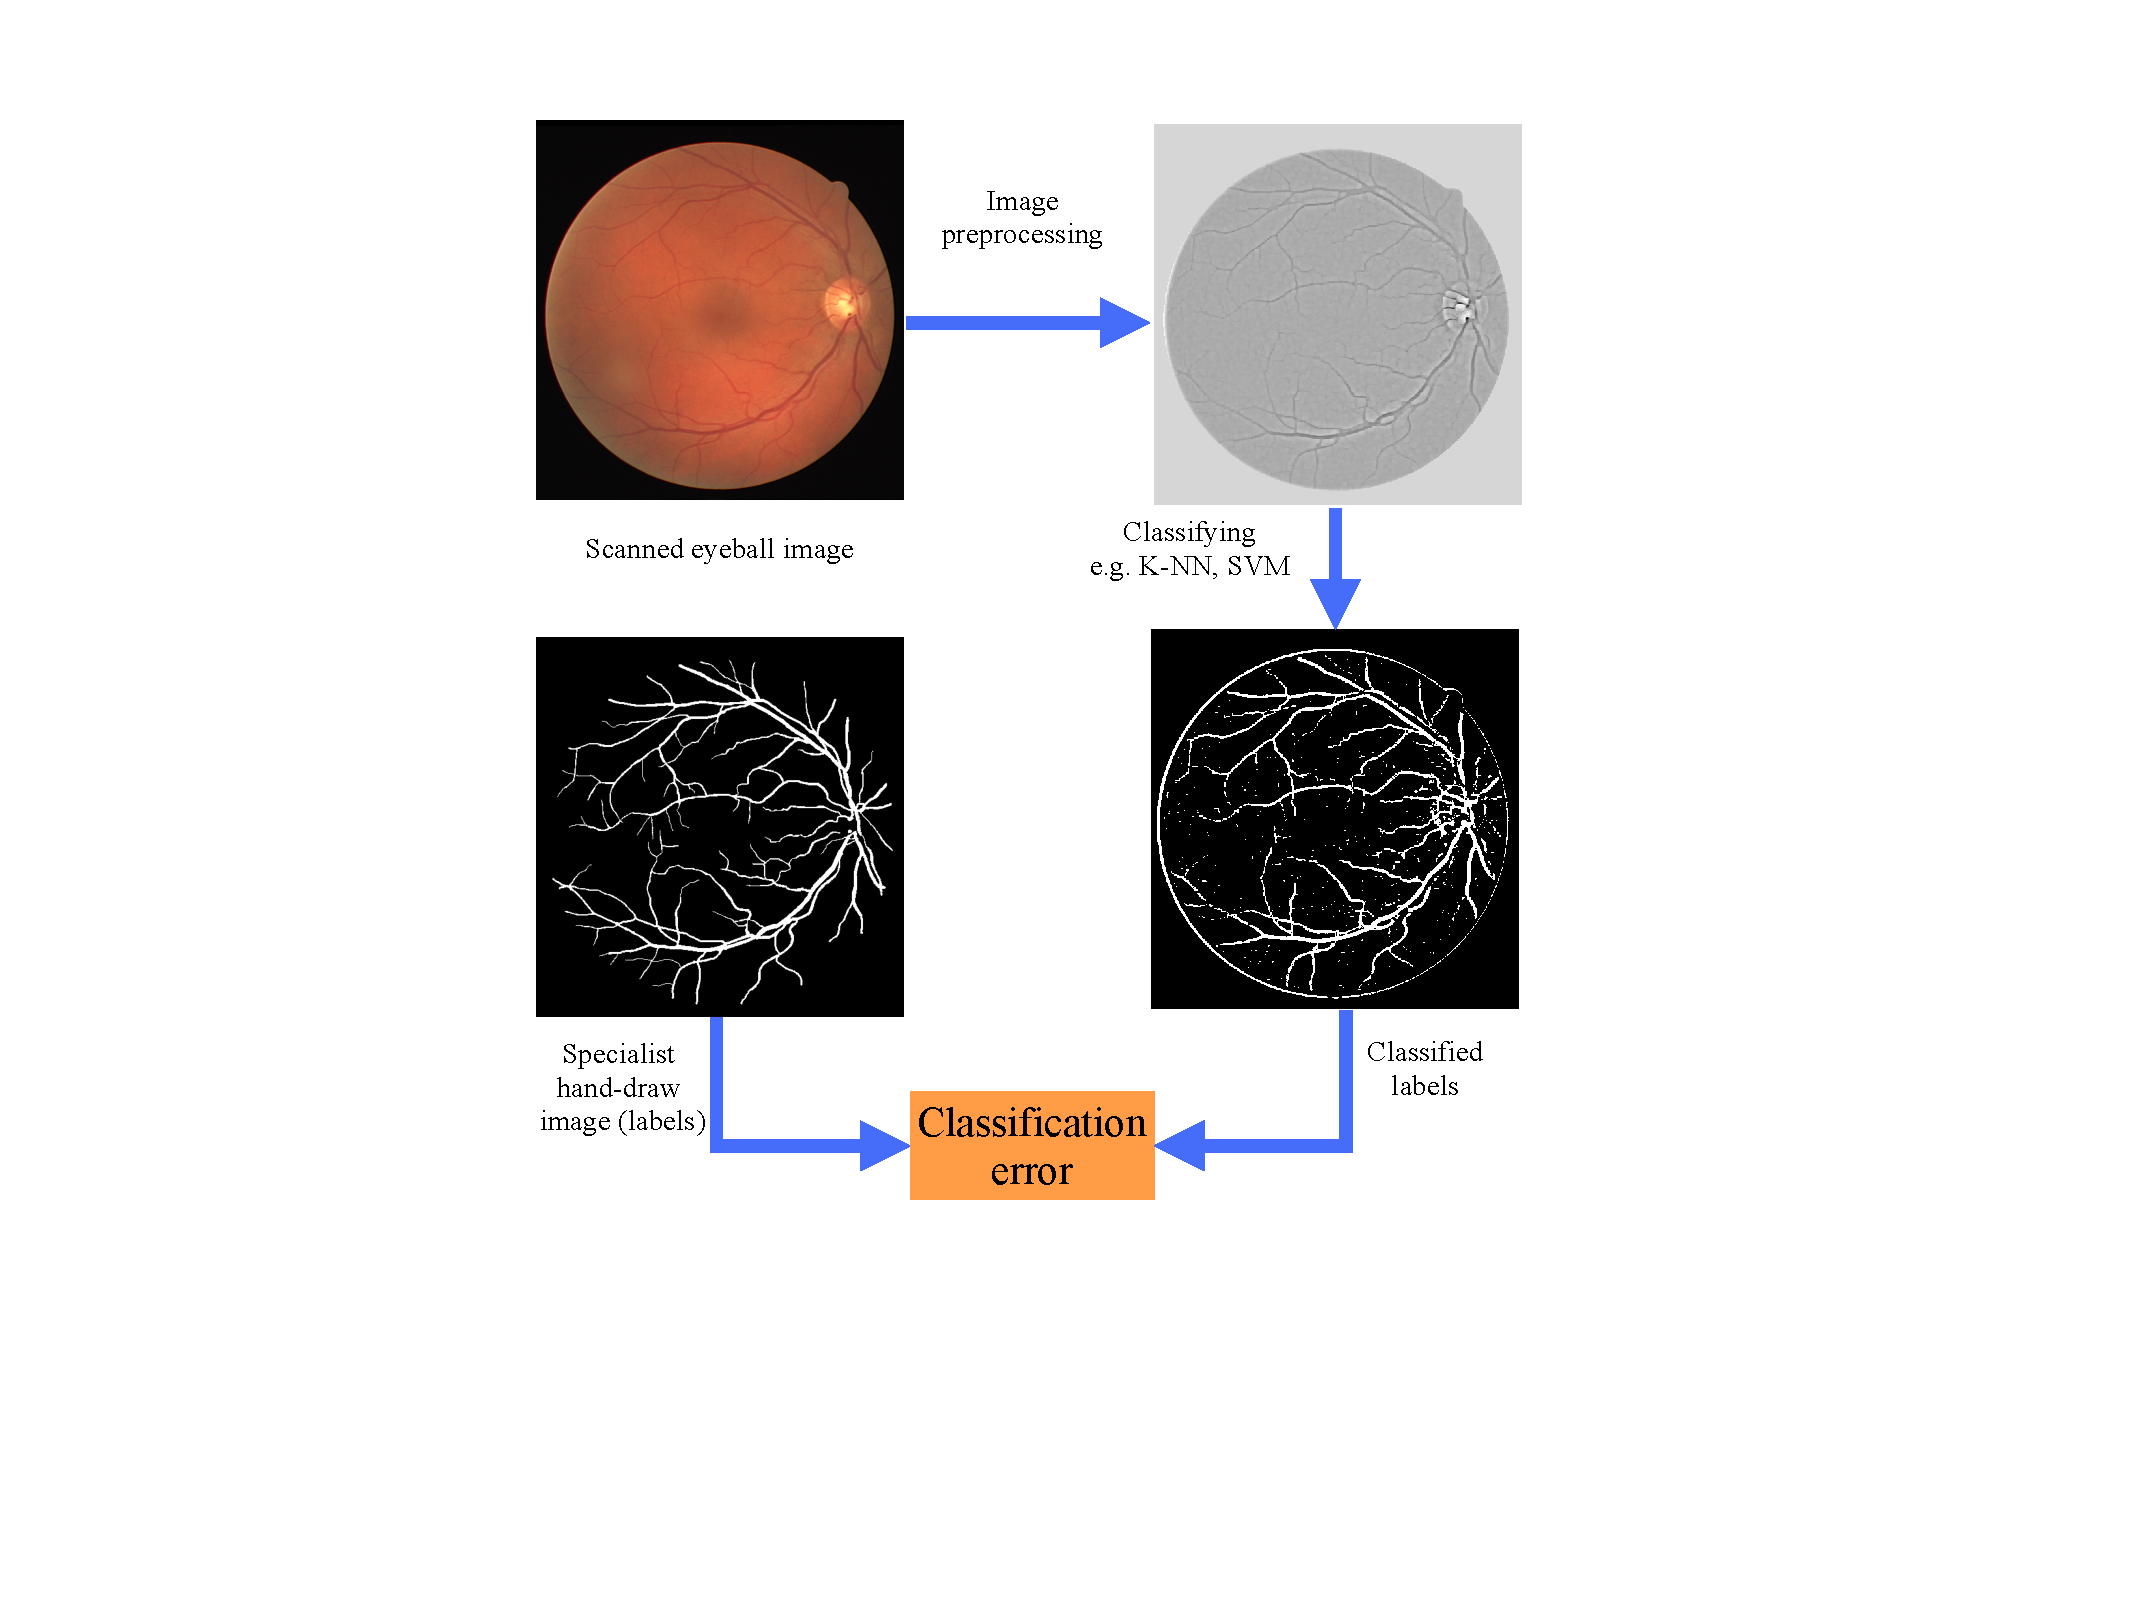
\includegraphics[width=0.8\columnwidth]{figures/procedure_project}
\caption{Procedures of the project}
\label{fig:procedure_project}
\end{figure}
  
%%% sec data src 
\section{Data Source and Image Preprocessing}  

The data used for this application is taken from a publicly available database DRIVE: Digital Retinal Images for Vessel Extraction \cite{staal2004ridge}.  There are raw scanned eyeball images of 40 patients, and the corresponding vessel-separated ones drawn by two specialists. (see \fref{fig:ex_eye_fig} for an example). Each image has a size of $584\times565$, a total of 329,960 pixels. Each pixel is an instance of data when training with machine learning method. There are two classes: vessel or background (non-vessel), and each pixel falls into one of the two categories.  The labels are obtained by inspecting the specialist's hand-drawn image, which is in a binary image, with values either 1 or 0.  The 40 images and the corresponding hand-drawn labels are divided equally into two groups, one of which is used as the training set and the other as test set.

%fig
\begin{figure}[H]
\centering
\begin{subfigure}{0.4\columnwidth}
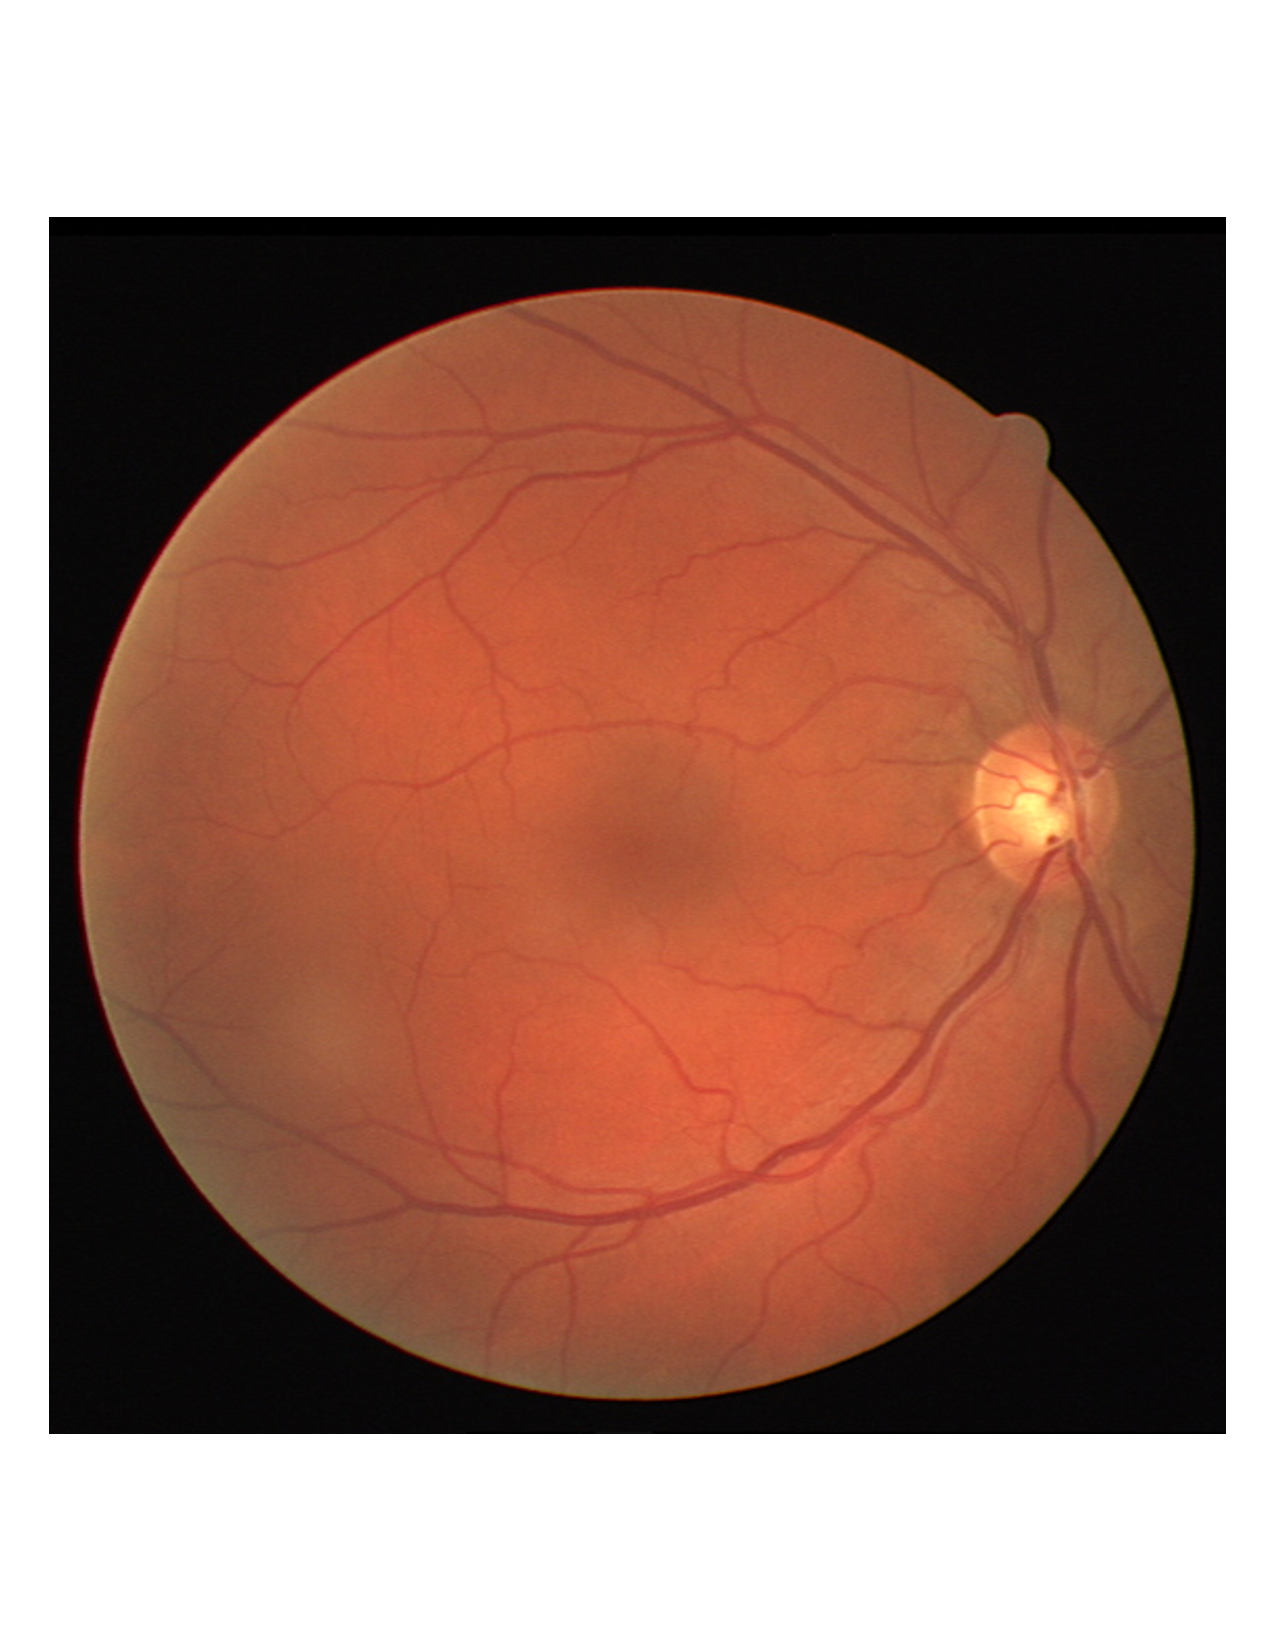
\includegraphics[width=\columnwidth]{figures/20_test}
\caption{}
\label{fig:}
\end{subfigure}
\begin{subfigure}{0.4\columnwidth}
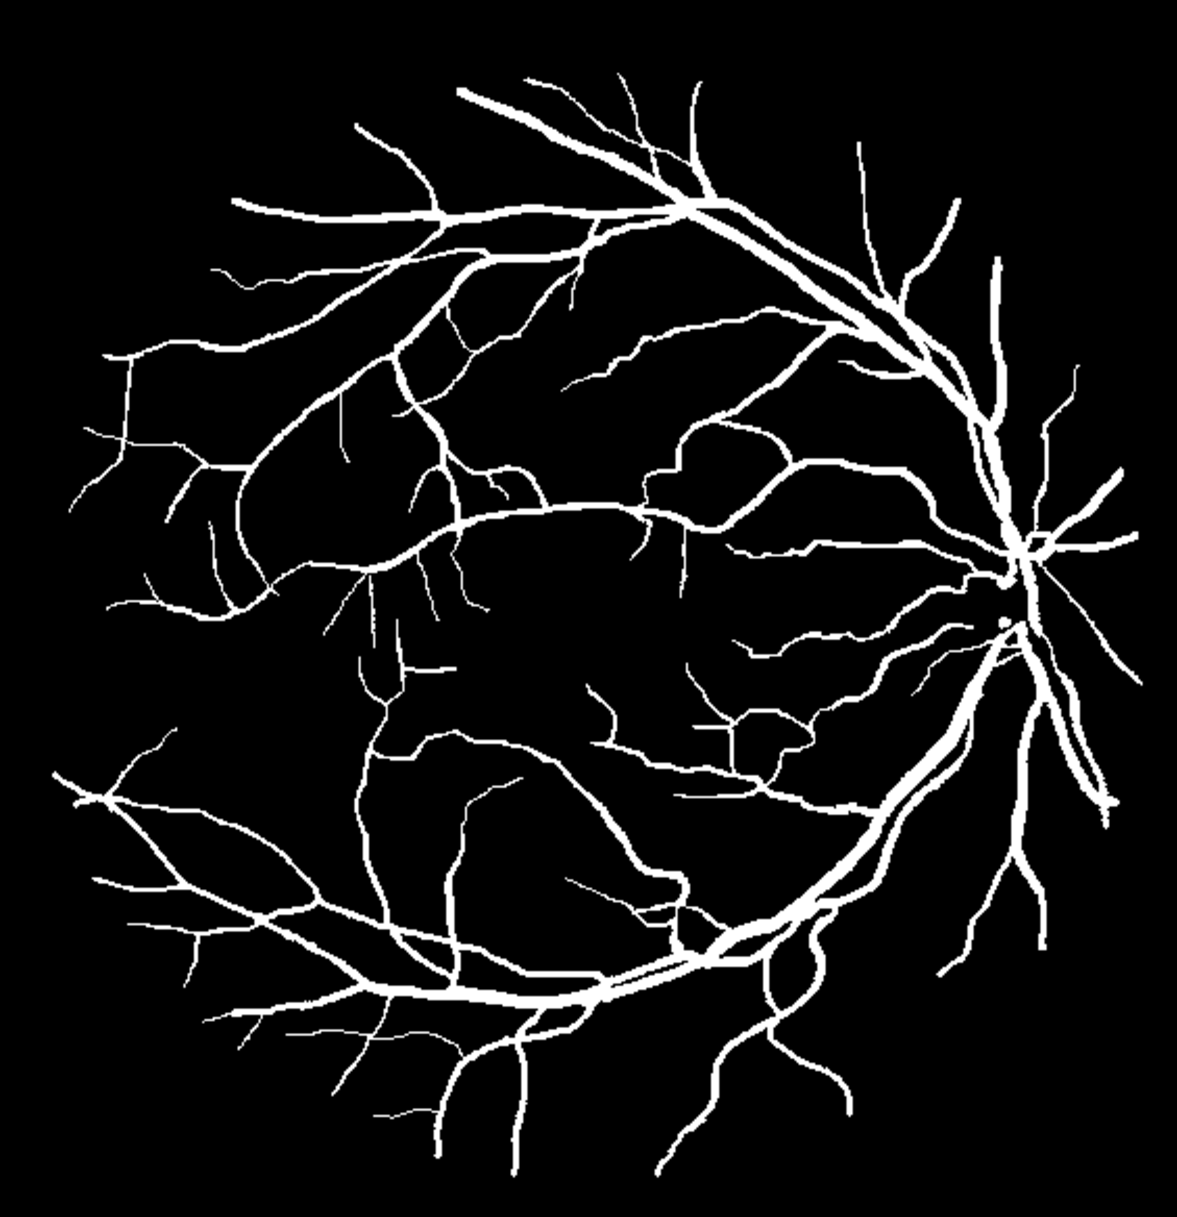
\includegraphics[width=\columnwidth]{figures/20_manual1}
\caption{}
\label{fig:}
\end{subfigure}
\begin{subfigure}{0.4\columnwidth}
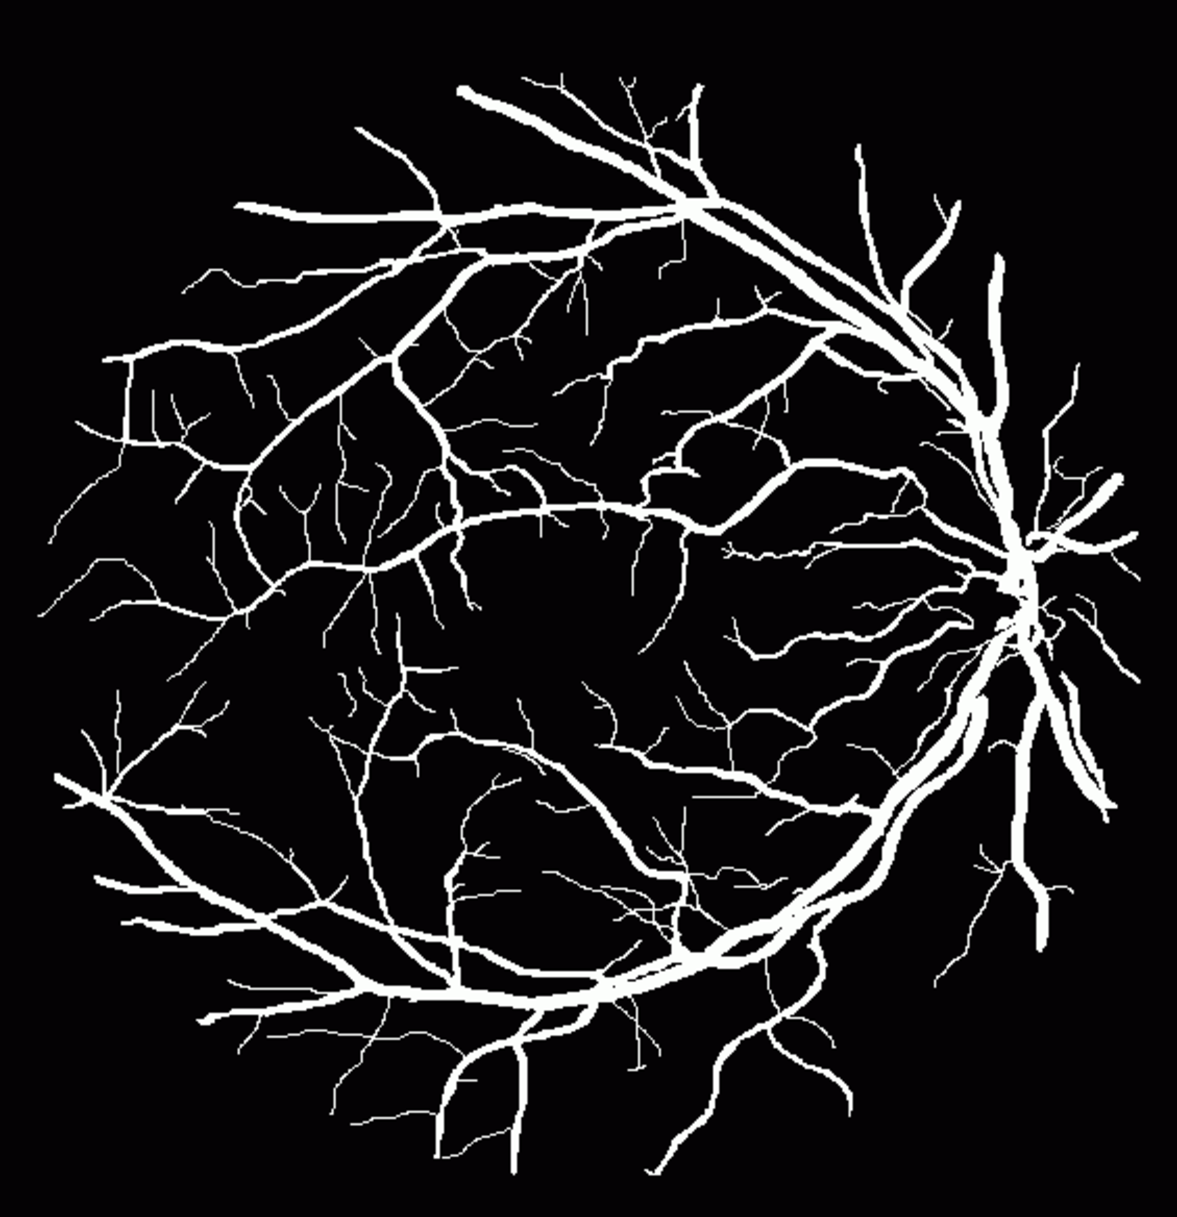
\includegraphics[width=\columnwidth]{figures/20_manual2}
\caption{}
\label{fig:}
\end{subfigure}
\begin{subfigure}{0.4\columnwidth}
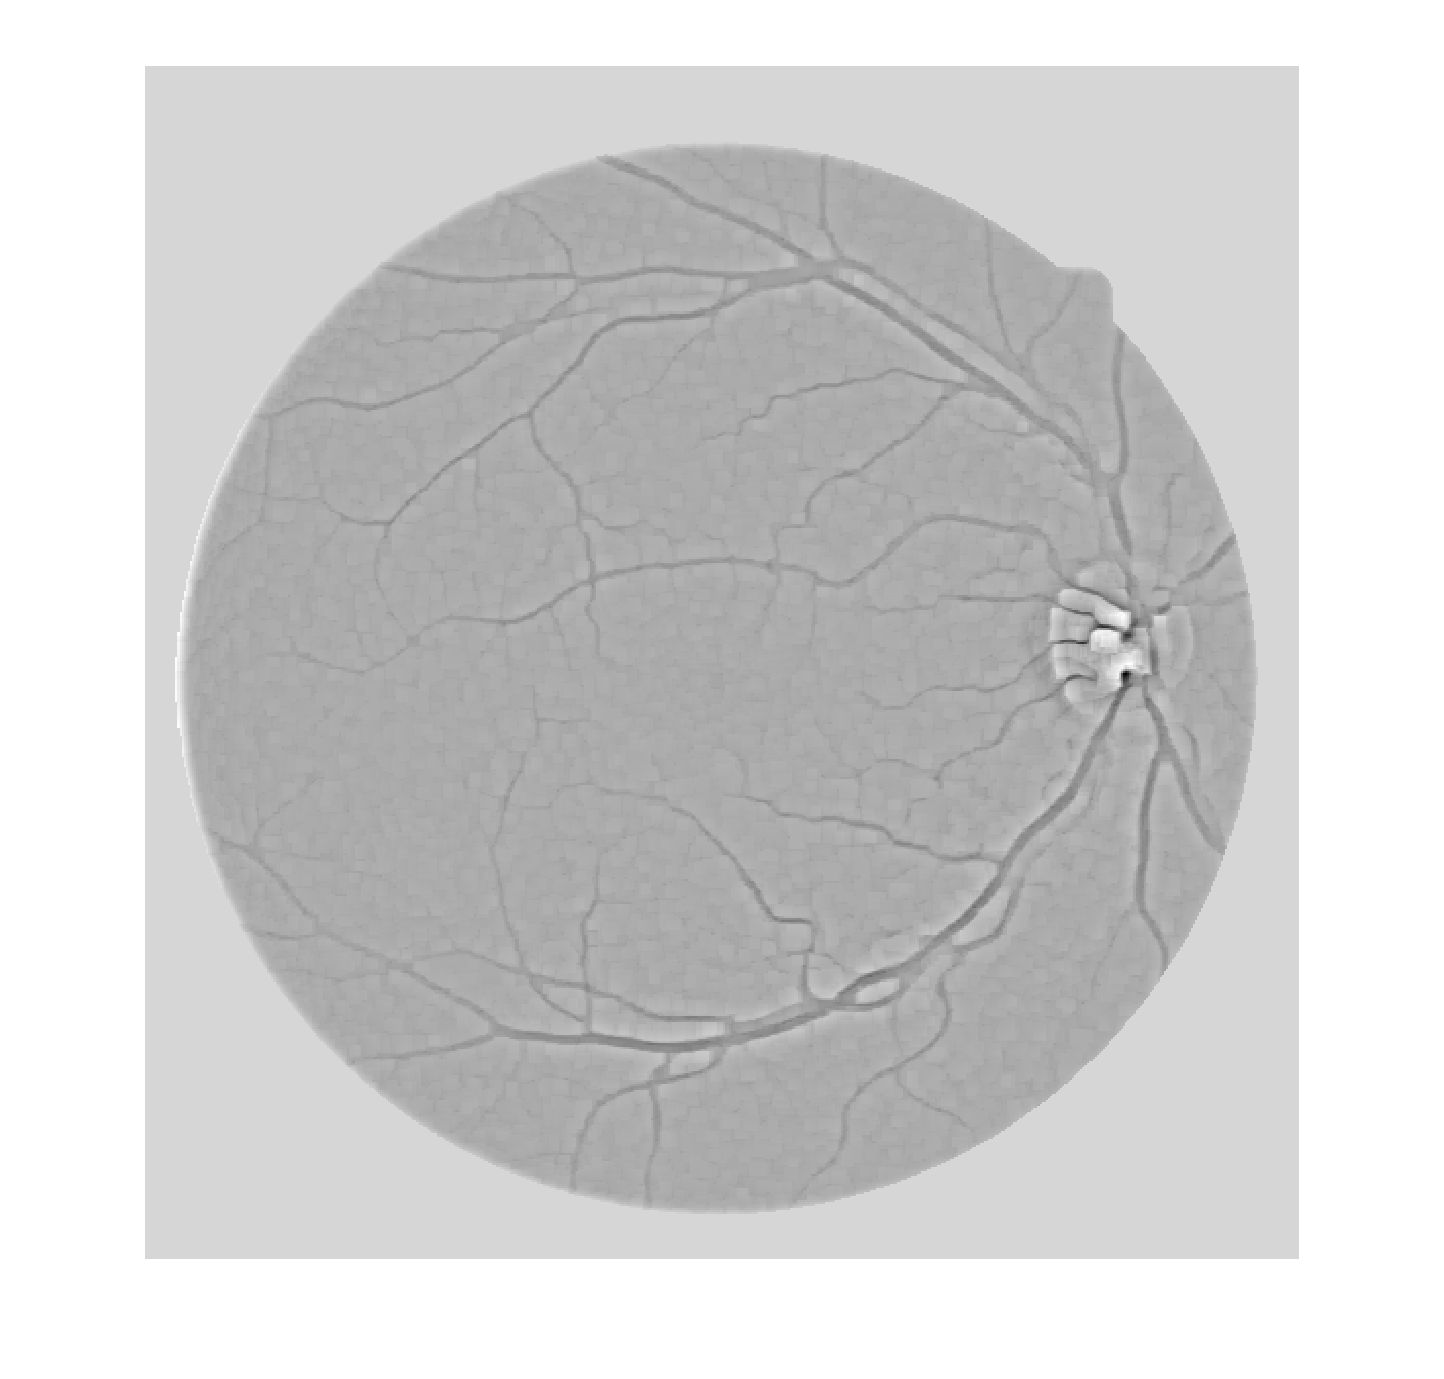
\includegraphics[width=\columnwidth]{figures/preprocessed_20}
\caption{}
\label{fig:after_preprocess}
\end{subfigure}
\caption{Example of an eyeball images. (a) Original scanned, (b) the corresponding hand-drawn one by first specialist, and (c) the corresponding hand-drawn one by second specialist. (d) The preprocessed image.}
\label{fig:ex_eye_fig}
\end{figure}
  


Before proceeding to input data into our classification machine, we need to implement a preprocessing process.  The pre-process is an important step in the retinal vessel segmentation procedure. The larger contrast between the vessel pixels and the background pixels, the better result will be produced by the machine learning classifier. Image processing is used in the pre-processing procedure. \verb|Matlab 2015b| is used to implement the image processing code for its powerful image processing toolbox and subroutines. The image processing procedure largely follows the procedure described in \cite{marin2011new}, and some small modifications are used to make the whole procedure more suitable for our application. 

The raw scanned eye image can be transferred to a RGB image first, then the green channel is extracted since the signal noise ratio is the largest in this channel \cite{marin2011new,ricci2007retinal}. The green-channel-only image is transformed into grayscale image for the easiness of classification.  The role of image processing is to remove the inhomogeneous illumination background of the eye ball.  For the geometric shape the eye, some part has stronger reflection than the others when an illumination is used. The image processing should not be used aggressively, since some information of the vessels might be lost in the image processing procedure.  An example of preprocessed image is shown in \fref{fig:after_preprocess}.




%%% sec: methodology 
\section{Methodology}

\subsection{Instance Features}

As mentioned in the above section, each pixel is treated as an instance in the data set. For each instance, we only have one feature (the intensity of the greyscale $I = I(x,y)$), which seems not to be enough to carry out the classification. The preprocessed image shows that the contrast of intensity between the vessel and the background is not very large, especially for those tiny vessels, which have a similar greyscale compared with the background. Therefore, we decided to include two more features: the magnitude of the gradient of intensity $F$,  and the largest eigenvalue of the Hessian of the intensity $\lambda$. $F$ and $\lambda$ can provide information for pixels near the boundary between vessels and background.  The magnitude of the gradient of intensity $F$ is obtained through:  
\begin{equation}
F = \sqrt{\left(\frac{\partial I}{\partial x}\right)^2 + \left(\frac{\partial I}{\partial y}\right)^2} . 
\end{equation}

The Hessian is:
\begin{equation}
H =
\begin{bmatrix}
  \frac{\partial^2I}{\partial x^2}   & \frac{\partial^2I}{\partial xy} \\
\frac{\partial^2I}{\partial xy}  &\frac{\partial^2I}{\partial y^2} 
\end{bmatrix} ,
\end{equation}
and as a results, the largest eigenvalue is:
\begin{equation}
\lambda = \frac{1}{2} \left( \frac{\partial^2I}{\partial x^2} +\frac{\partial^2I}{\partial y^2} + \sqrt{\left(\frac{\partial^2I}{\partial x^2} - \frac{\partial^2I}{\partial y^2} \right)^2 + 4 \left( \frac{\partial^2I}{\partial xy} \right)^2 } \right) \,.
\end{equation}

All the partial derivatives are evaluated numerically using \verb|imgradientxy| in \verb|matlab|. Actually, there are other features that can be assigned to each data instance.  In order to reduce the computational cost while keeping as much information as possible, we only use $I$, $F$, and$\lambda$ as the features in the training and test data set \cite{alex2014machine}.

 
% knn
\subsection{K-Nearest Neighbor}

We used K-nearest neighbor (K-NN) as a supervised learning method to classify the instances (pixels) by using the specialist's hand-drawn images as the label in the training set. The basic idea of K-NN is straightforward. To classify an instance, the ``closest'' k instances in the training set are picked out by the algorithm.  The dominant label of the k instances determines the label of instance to be classified.  The ``closeness'' is defined as the similarity between two pixels, and weighted Euclidean distance is used here to measure the similarity,
\begin{equation}
d = \sqrt{ w_I\cdot I^2 + w_F\cdot F^2+w_\lambda \cdot \lambda^2} ,
\end{equation}

where $w_I$, $w_F$ and $w_\lambda$ are the weights. The weights are chosen such that the intensity $I$, the gradient $F$, and the largest eigenvalue $\lambda$ contribute equally to the distance. As an indication of similarity, smaller the distance between two pixels, more similar they are. This is a two-class case, where a test instance will be either classified as 1 or $-1$. 

One of the key components to use K-NN is to choose the appropriate number of neighbors K.  After playing with the parameters, we found that in the case $K=800$ gave a good results.  So both in the classic K-NN and the modified K-NN (discussed in the next section),  $K=800$ is choosen.

K-NN is a method requiring a large amount of computational effort. Each instance in the testing set will be compared with all the instances in the training set to find the ``closest'' K neighbors. In our case, for one testing image the complexity will be $O(329960)$, which is a very large number. 
 
% modified knn
\subsection{Modified K-NN}\label{sec:modi_knn}

Modified K-NN is basically the same as the classic K-NN as described above.  The only difference is that when the K nearest neighbors are found in the algorithm, instead of choosing the dominant labels as the label of training set, these greyscale of the K nearest neighbors are averaged to obtain the new value for the test instance. In such a way, modified K-NN becomes an unsupervised method.  

For the work of blood vessel segmentation, the ultimate goal is to show the image clearly and keep as much information as possible so the doctor can make correct decisions based on the image. There is no need to set a stiff boundary between the vessel and the background.  The final image is then a continuous greyscale image, a doctor can see the small vessels better compared with the classic K-NN method.  However, the error rate is not easy to estimate in this case since the blood vessels are not really classified in this method. 

% svm
\subsection{Support Vector Machine}

Compared with K-NN, Support Vector Machine (SVM) costs less computational resources.  SVM tries to find the optimal boundary between two classes of the training set: vessel and background. The optimal boundary is the one that maximize the margin between these two classes.  

Ideally, the margin is $1/|w|$ in the classic SVM method.  However, the classic SVM method does not work well for the linear inseparable data. When the data are not be able to separate linearly, a soft margin method is introduced \cite{veropoulos1999controlling, ricci2007retinal}, where we need to maximize 
\begin{equation}
g = \frac{1}{2}\boldsymbol{w}^T\boldsymbol{w} + C^+ \sum_{i \,|\, yi = +1} \xi_i + C^- \sum_{i \,|\, yi = -1} \xi_i
\end{equation}
under the constraints, 
\begin{equation}
\begin{aligned}
y_i(\boldsymbol{w}^T\boldsymbol{x}_i + b ) &\geq 1 - \xi_i, \quad i = 1,\ldots, N\\
\xi &\geq 0, \quad\quad\quad  i = 1,\ldots, N
\end{aligned}
\end{equation}

where $\xi$ are the slack variables.  The margin in the soft margin method is smaller compared with the classic method, which means the method allows the existence of some misclassified data points. $C^+$ and $C^-$ are the parameters set by the user. When $C^+$ is larger, less misclassified positive points will be found; when $C^-$ is larger, less misclassified negative points will be found. 

We've tried to code the SVM in \verb|Matlab|, but the results obtained by our code is not so good. So we turned to an python based machine learning package \verb|PyML| \cite{pyml}. This package allows the user to set the values of $C^+$ and $C^-$. We set them based on \eqnref{eq:c}.
\begin{equation}\label{eq:c}
\begin{aligned}
&C^+ + C^- = 1 \\
&\frac{C^+}{C^-} = \frac{\text{number of instances with label = 1}}{\text{number of instances with label = -1}}  \\
\end{aligned}
\end{equation}



%%% results
\section{Results}

The ultimate goal of the vessel segmentation is to obtain vessel images as clear as possible.  The classified labels of the instances (pixels) of a test set need to be transferred to images people can view.  The process is pretty simple. For classic K-NN and SVM methods, the label -1 and 1 are transferred to 0 and 1, respectively, and then 0 and 1 are used to generate greyscale binary images.  For the modified K-NN, we can just plot the classified labels recalling that the classified labels are averages of the greyscale intensity of K nearest neighbors. 


As mentioned above, each image has 329,960 data instances.  For K-NN the computational time is quite long provided we use \verb|Matlab|.  The code was run on a machine with 32 kB L1, 256 kB L2, and 8 MB L3 caches and 3 GB RAM, and it takes about 6 hours to finish. Therefore, we only include one image in the training set, and use another image as as test set. 

The classified results of the three methods investigated in the report are presented in \fref{fig:rslt}. It is seen that the basic features of the vessels are all well captured, although some discontinuity are observed, especially in the tiny vessels. But we note that the discontinuity is not so obvious in the image using modified K-NN method. This is largely because there is no hard boundary between vessels and the surrounding background. 
 

%fig
\begin{figure}[H]
\centering
\begin{subfigure}{0.4\columnwidth}
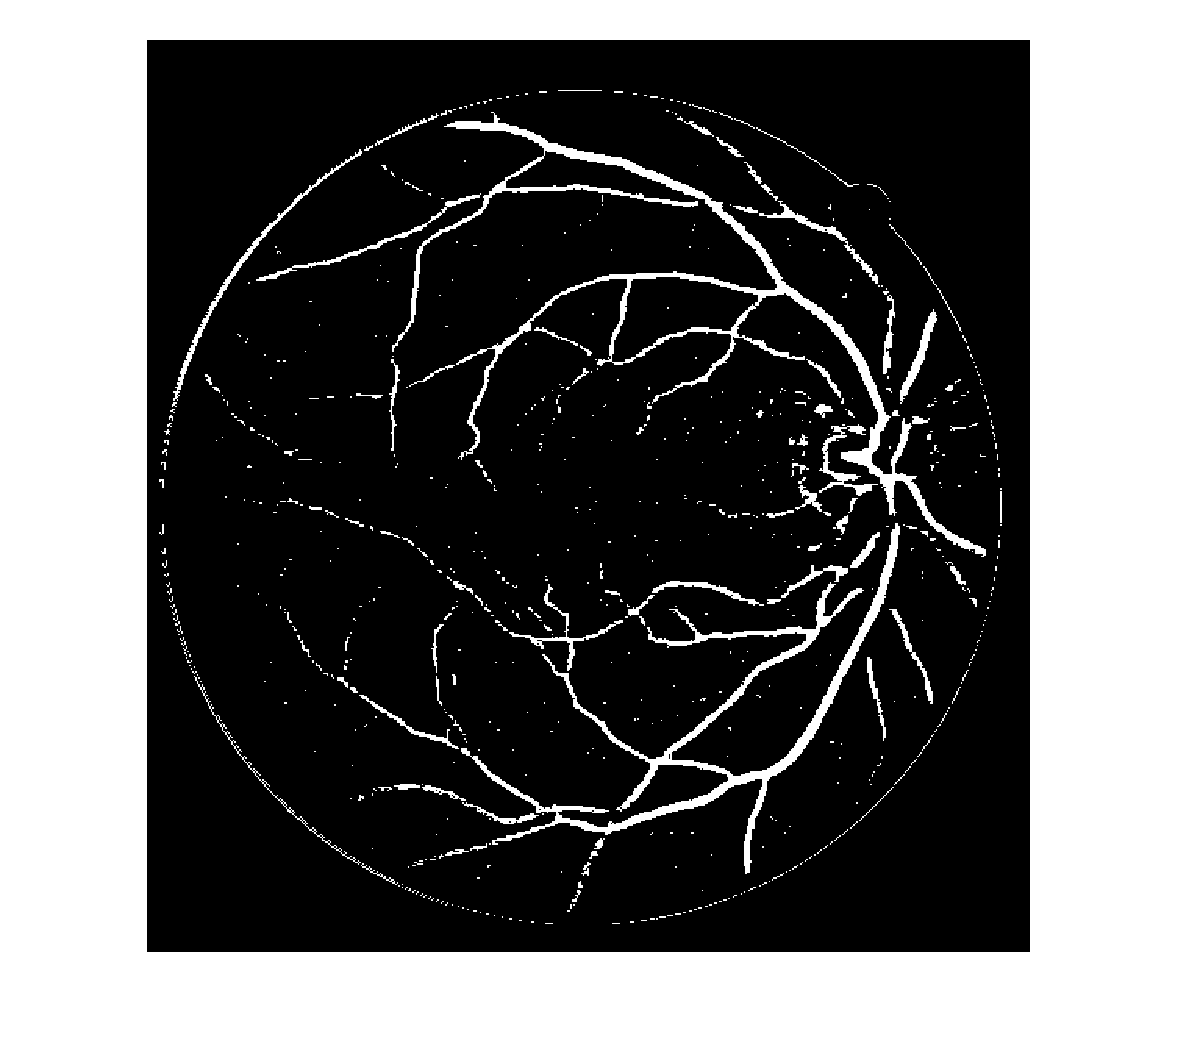
\includegraphics[width=\columnwidth]{figures/rslt_knn}
\caption{}
\label{fig:}
\end{subfigure}
\begin{subfigure}{0.4\columnwidth}
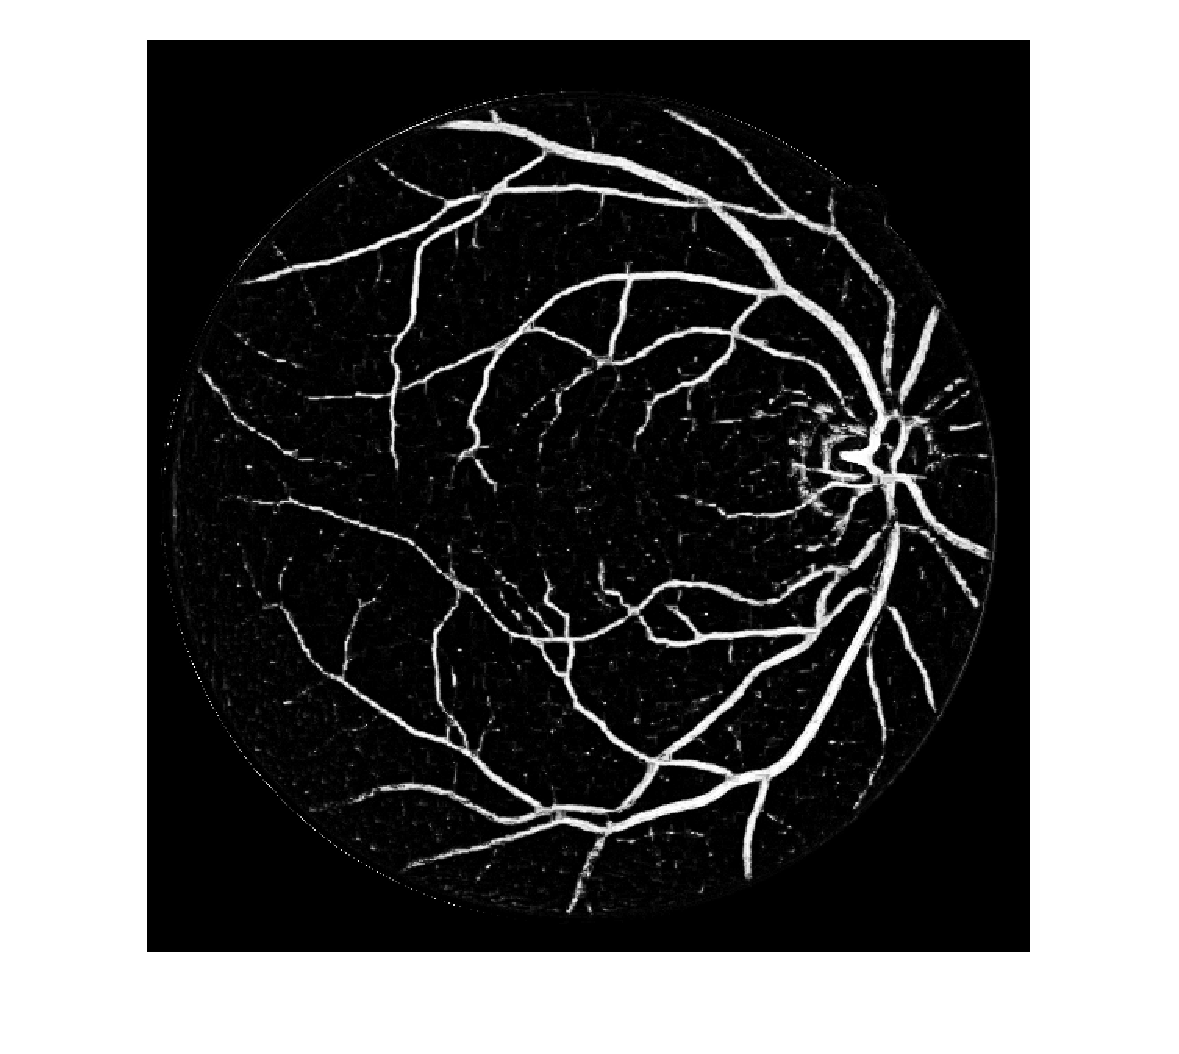
\includegraphics[width=\columnwidth]{figures/rslt_knn_mean}
\caption{}
\label{fig:}
\end{subfigure}
\begin{subfigure}{0.4\columnwidth}
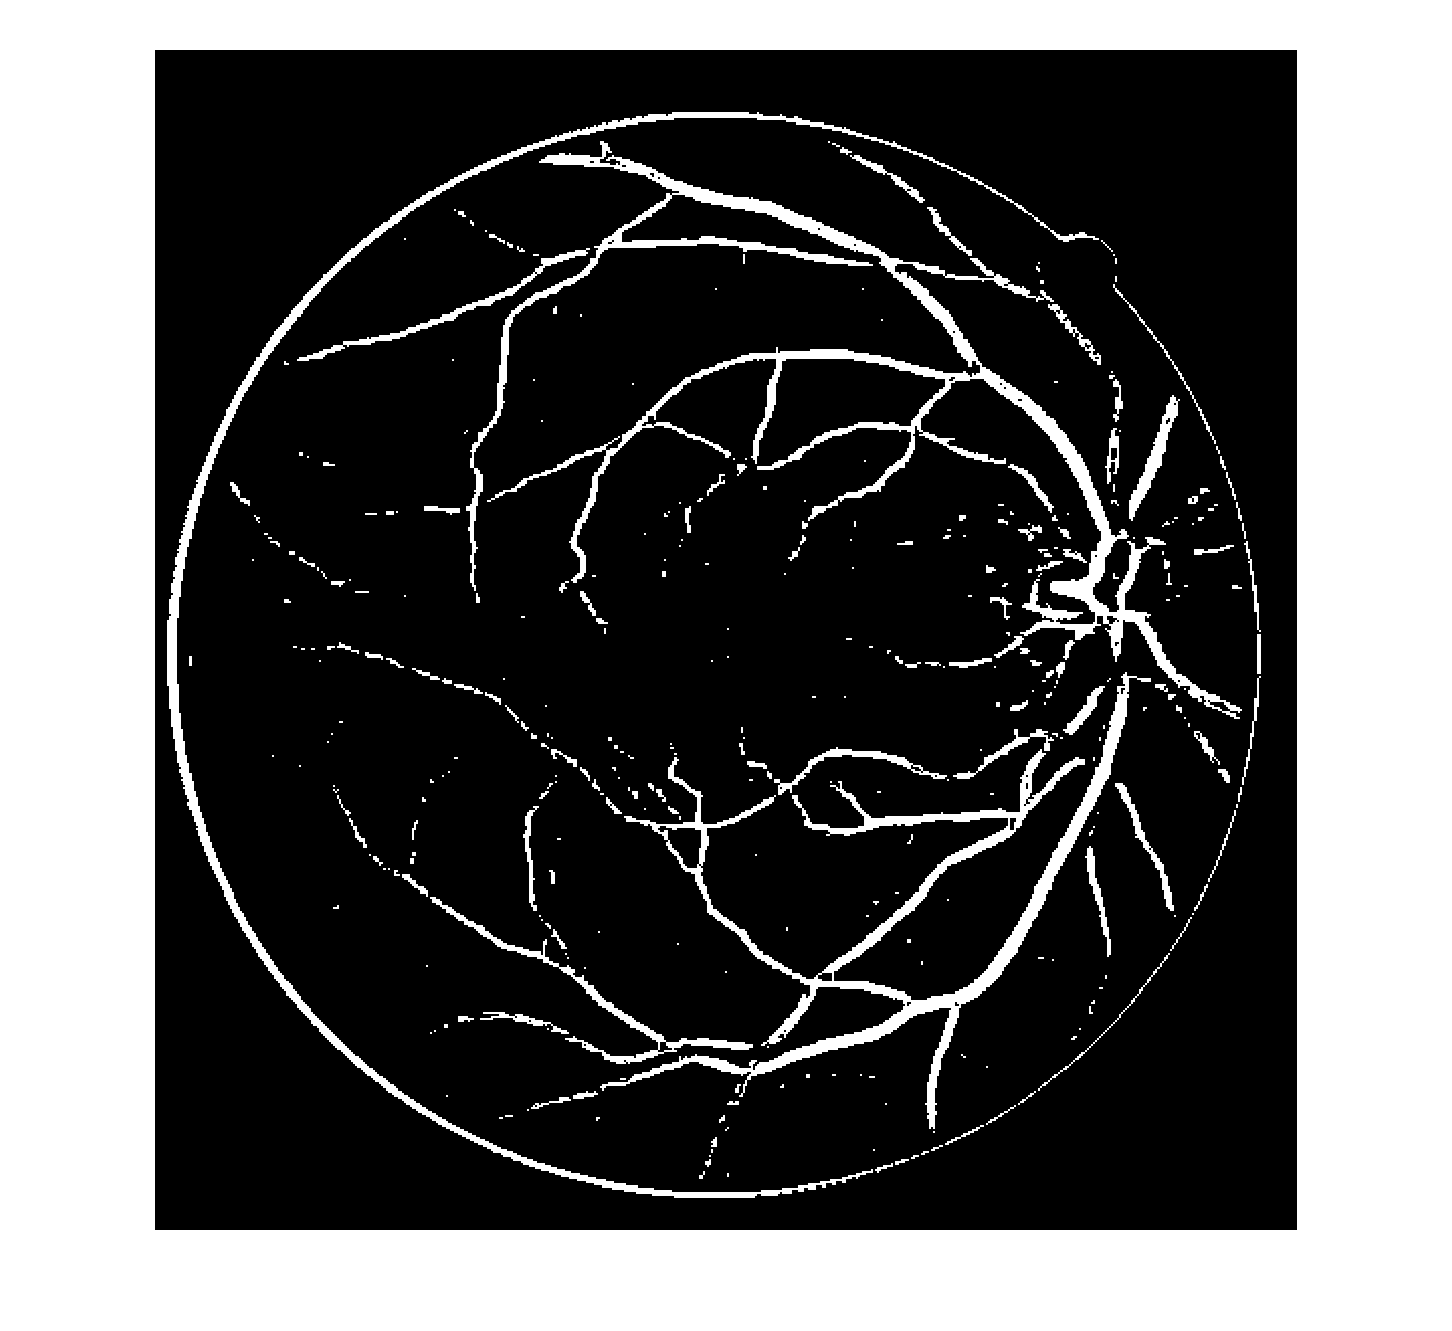
\includegraphics[width=\columnwidth]{figures/rslt_svm_better_6}
\caption{}
\label{fig:}
\end{subfigure}
\caption{Classified images trained using (a) classic K-NN, (b) modified K-NN, and (c) SVM.}
\label{fig:rslt}
\end{figure}
  


To quantitatively investigate the classification methods, we need to compute the classification error or accuracy rate. They are defined as follows:
\begin{equation}
\begin{aligned}
Error &= \frac{\text{\# Misclassified pixel}}{\text{\# Total pixel}} = \frac{\sum_{i=1}^N|y_i - C_i|}{2N} \\
Accuracy &= 1- \frac{\text{\# Misclassified pixel}}{\text{\# Total pixel}} = 1- \frac{\sum_{i=1}^N|y_i - C_i|}{2N} \\
\end{aligned}
\end{equation}
where, $N$ is the number of pixels in an image (i.e.  329,960), $y_i$ is the label obtained from the specialist's hand-drawn image, and $C_i$ is the classified label. Note that the 2 is included in the denominator because the labels have discrete values of -1 and 1, not 0 and 1. 

As mentioned in Section~\ref{sec:modi_knn}, we cannot compute the error or accuracy for the modified K-NN method since the where the labels are obtained by averaging over the K nearest neighbors. They are not discrete values -1 and 1, and if we compute the error rate, it would be quite large even though modified K-NN yields a little bit better classified image than the other two methods. 


\tabref{tab:class_error_knn} lists the classifications errors for the classic K-NN method and the SVM method.  For example, for the $\#06$ image using K-NN, there are 20,204 pixels misclassified, and therefore the error rate is $20,204/329,960= 6.12\%$. The error rate is $18,722/329,960 = 5.67\%$ if SVM is used. 

The error rate is mainly caused by the misclassification of tiny vessels. After preprocessing, these tiny vessel almost has the same greyscale value as the background. Consequently, it is difficult to separate them from the background. Another source for the error is the outer ring that corresponds to the shape of the eyeball as seen in panel (a) and (c) of \fref{fig:rslt}. 

% table 
\begin{center}
\captionof{table}{Classification Error}
\label{tab:class_error_knn}
\begin{tabular}{c c c c c}
\hline
\hline
image number          & 06   &   10  &  15     \\
\hline
classical K-NN  & 6.12\%  &6.83\% & 5.92\%    \\
SVM             & 5.67\%  &6.22\% & 5.73\%    \\
\hline
\hline
\end{tabular}
\end{center}


%%%discussion
\section{Discussion}

In this report, we have implemented three machined learning methods (K-NN, SVM and modified K-NN) to classify the retinal vessels images. Basically, they yield the same level of accuracy. The error rate of SVM is a little bit smaller compared with classic K-NN.  The continuity of tiny vessels is better using the modified K-NN method.   

The SVM is designed to find the maximum margin between two classes. Considering the complexity of the application here, a soft margin is used.  In such a way, SVM will always produce a satisfactory result. However, our results show that SVM cannot eliminate the discontinuity of some tiny vessels.  It is largely due to the preprocessing process where the greyscale of the tiny vessel becomes quite similar to the background.  The results of SVM may be improved by (i) choosing appropriate $C^+$ and $C^-$; (ii) using nonlinear kernels, such as polynomial.  

K-NN yields good results as well, but it needs much more computational resources. In order to improve the result of K-NN, a modified version is put forwards, where the greyscale of a pixel is obtained by averaging the greyscale of the K nearest neighbors. The modified K-NN method does not use any boundary between vessel and background at all.  Other ways to improve the K-NN results includes changing the definition of distance. As a result, different features can have different contribution to the distance. We suspect that the greyscale integrity $I$, and the gradient magnitude $F$ should have a larger weight than the largest eigenvalue of the Hessian $\lambda$ if we want to get better results. But this remains verification. 


Other general ways to improve the results includes:
\begin{enumerate}
\item Increase the size of training set. Considering the computational time, we only use one image as the training set. A better classification results can be achieved if we increase the number of images used in the training set. 
\item Employ more advanced image processing techniques.  We can remove the ring that corresponds to the shape of the eyeball.  Also, the contrast between the tiny vessels and the background could be made larger.  
\item  More features can be assigned to each pixel to get a better description of its characteristics given enough computational power.
\item Different weight in the distance function should be tried and tested to find the optimal values. 
\item Post-processing can be used to get a more clear image by removing the outer ring and other noise left in the image after the process of machine learning algorithm.
\end{enumerate}



%%% appendix
\newpage
\appendix
\section{How to Run the Code}
\label{appendix:a}

All the codes are included in the \verb|code| directory, where the K-NN and SVM codes are in \verb|code/knn| and \verb|code/svm|, respectively. 

The following files are in the \verb|code/knn| directory:
\begin{itemize}
\item \verb|read_img.m|: reading in the eyeball image;
\item \verb|bg_homo.m|: preprocessing the image;
\item \verb|generate_data_set.m|: generating instance features $I$, $F$ and $\lambda$.
\item \verb|generate_label.m|: generating label data;
\item \verb|k-nn.m|: K-NN algorithm;
\item \verb|classify_error.m|: calculating classification error;
\item \verb|vessel_diagnosis.m|: the main program, which calls the functions to preprocess images, run K-NN, compute classification error, and output classified image. 
\end{itemize}

To run the K-NN code, just double click \verb|vessel_diagnosis.m| to open it with \verb|Matlab2015| and then run it. Note that this code may not work on some lower version of \verb|Matlab| because the image processing toolbox is not available.

The following files are in the \verb|code/svm| directory:
\begin{itemize}
\item \verb|read_img.m|, \verb|bg_homo.m|, \verb|generate_data_set.m|, \verb|generate_label.m|, \verb|classify_error.m| are the same as those in the \verb|code/knn| directory; 
\item \verb|generate_svm_data.m|: output training data, training label and test data to be used by \verb|PyML|;
\item \verb|main.m|: wrapper to generate data for SVM use.
\item \verb|svm.py|: SVM classification via \verb|PyML|;
\item \verb|plot_results.m|: plot the classified labels. 
\end{itemize}


To run the SVM code, the \verb|PyML| package needs to be installed. Then do the following:
\begin{enumerate}
\item  \verb|% cd code/svm|
\item double click \verb|main.m| and run it to generate the training set, and test set
\item run the SVM classification by:  \\
\verb|% python svm.py|
\item double click \verb|plot_results.m| and run it to plot
\end{enumerate}

The code for the modified K-NN is almost the same as for the K-NN code. We just need to comment lines 25 and 26 and uncomment line 29 in the \verb|knn.m| file and then run it in the same way as the K-NN code.




%%% bibliography
\newpage
\bibliography{bib_machine_learning_project.bib}
\bibliographystyle{unsrt}
%\bibliographystyle{IEEEtran}


\end{document}  











%single figure
\begin{figure}[H]
\centering
\includegraphics[width=0.6\columnwidth]{}
\caption{  }
\label{fig:}
\end{figure}

%single figure
\begin{center}
\includegraphics[width=0.6\columnwidth]{}
\captionof{figure}{}
\label{fig:}
\end{center}

%subfigures
\begin{figure}[H]
\centering
\begin{subfigure}{0.48\columnwidth}
\includegraphics[width=\columnwidth]{}
\caption{}
\label{fig:}
\end{subfigure}
\begin{subfigure}{0.48\columnwidth}
\includegraphics[width=\columnwidth]{}
\caption{}
\label{fig:}
\end{subfigure}
\begin{subfigure}{0.48\columnwidth}
\includegraphics[width=\columnwidth]{}
\caption{}
\label{fig:}
\end{subfigure}
\begin{subfigure}{0.48\columnwidth}
\includegraphics[width=\columnwidth]{}
\caption{}
\label{fig:}
\end{subfigure}
\caption{bla.(a)bla. (b) bla. (c) bla. (d) bla.}
\label{fig:}
\end{figure}



% subfigure
\begin{minipage}[b]{0.49\columnwidth}
\begin{center}
\includegraphics[width=1\columnwidth]{D_with_T_at_F1_pts500}
  \captionof{figure}{at F=1 and \# pts=500 }
\end{center}
\end{minipage}
\hspace{0.02\columnwidth}
\begin{minipage}[b]{0.49\columnwidth}
\begin{center}
\includegraphics[width=1\columnwidth]{relative_error_D_with_T_at_F1_pts500}
  \captionof{figure}{Corresponding relative error }
\end{center}
\end{minipage}



% table with bold line header  need to use `booktabs' package 
%table
\begin{table}[h]
\caption{caption}
\label{tab:}
\centering
\begin{tabular}{lcr}
\toprule
        &        &      \\
\hline
        &        &      \\
        &        &      \\
        &        &      \\
\toprule
\end{tabular}
\end{table}


% table with double line header

% table 
\begin{center}
\captionof{table}{}
\label{tab:}
\begin{tabular}{c c c c c}
\hline
\hline
    &    &    &    &     \\
\hline
    &    &    &    &     \\
    &    &    &    &     \\
    &    &    &    &     \\
\hline
\hline
\end{tabular}
\end{center}





%table    multicolumn 
\begin{table}[h]
\caption{caption}
\centering
\begin{tabular}{lcr}
\hline
\multicolumn{2}{c}{Item} \\
\cline{1-2}
   a     &  e      &  i    \\
\hline
   b     &   f     &   j   \\
   c     &    g    &   k   \\
   d    &     h   &    l  \\
\hline
\end{tabular}
\end{table}




